%! TeX program = xelatex
\documentclass{article}
\usepackage[version=4]{mhchem}
\usepackage{fontspec}
\usepackage{graphicx}
\usepackage{tikz}
\usepackage{hyperref}
\usepackage[normalem]{ulem}
\usepackage[margin=0.75in]{geometry}

\graphicspath{{../}, {../../}}
\hypersetup{
  colorlinks   = true,
  urlcolor     = blue,
  linkcolor    = blue,
  citecolor   = red
}

\setmainfont{Noto Serif CJK KR}
\title{산화 환원 반응에서의 산화수}
\author{
    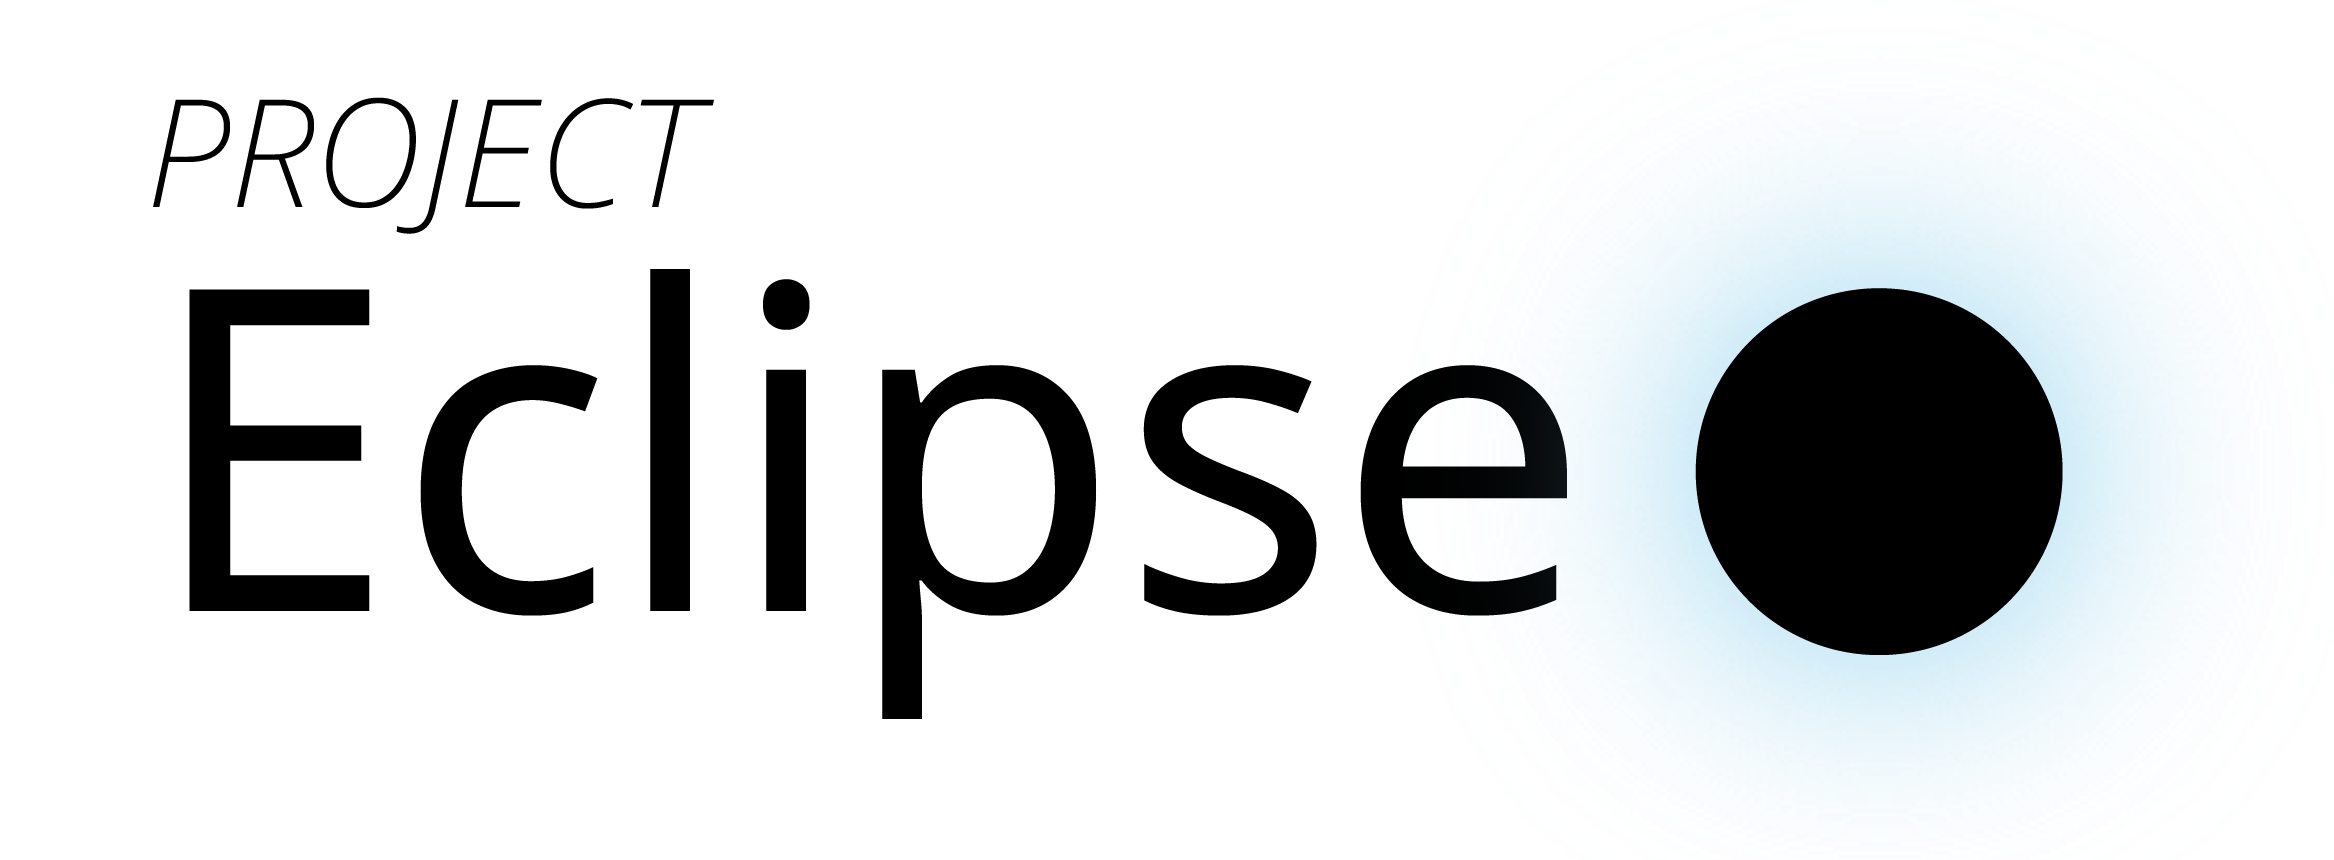
\includegraphics[scale=0.25]{logo}
}
\date{}

\begin{document}
\maketitle

\section{중학교, 통합과학 수준에서의 산화 환원 반응의 설명}

\subsection{산소의 이동을 이용한 설명}
중학교 과학에서, 산화 환원 반응은 산소의 이동으로 설명했습니다. 예를 들어 간단한 화학 반응인 구리의 산화 반응을 봅시다.

\[
    \ce{2CuO + C -> 2Cu + CO_2}
\]

산화는 산소를 얻는 반응, 환원은 산소를 잃는 반응이므로 이 반응식에서 \ce{C}는 산회되고, \ce{CuO}는 환원된다고 배울 겁니다. 여기까지는 간단합니다. \newline

그렇다면, 이런 반응은 어떨까요?

\[
    \ce{Cu^{2+} + Zn -> Cu + Zn^{2+}}
\]

산소의 이동으로 이 반응을 설명할 수는 없습니다. 화학식에서 볼 수 있듯 이 반응에서 산소는 관여하지 않거든요! 그러면 이 반응을 어떻게 설명할까요?

\subsection{전자의 이동을 이용한 설명}
앞서 나온 반응처럼, 산소가 관여하지 않는 산화 환원 반응을 설명하기 위해, 통합과학에서는 전자의 이동을 이용합니다. \newline

반응에서 \ce{Cu^{2+}}는 다음과 같이 전자를 얻어 \ce{Cu}가 됩니다. \sout{CU가고싶다}

\[
    \ce{Cu^{2+} + 2e^- -> Cu}
\]

또한, \ce{Zn}은 다음과 같이 전자를 잃고 \ce{Zn^{2+}}가 되죠.

\[
    \ce{Zn -> Zn^{2+} + 2e^-}
\]

따라서 앞서 나온 구리와 아연의 반응식에서

\[
    \ce{Cu^{2+} + Zn -> Cu + Zn^{2+}}
\]

산화되는 물질은 \ce{Zn}이고, 환원되는 물질은 \ce{Cu^{2+}}입니다. 이처럼 전자의 이동을 사용하면, 산소의 이동보다 더 많은 종류의 산화 환원 반응을 설명할 수 있습니다. 하지만 과연 그 정도로 쉽게 끝날까요?

\subsection{공유 결합 물질의 화학 반응}
다음 화학 반응식을 봅시다.

\[
    \ce{CH_4 + 2O_2 -> CO_2 + 2H_2O}
\]

많은 통합과학 참고서에서 등장하는, 메테인의 연소 반응입니다. 여기서 어떤 물질이 산화되고, 어떤 물질이 환원되었을까요? 답은 ``\ce{CH_4}가 산화되었고, \ce{O_2}가 환원되었다.'' 입니다. 그런데, 어떤 근거로 그렇게 주장할 수 있을까요? 화학 반응식에서 볼 수 있듯 산소만 이동한 것이 아니므로 산소의 이동으로는 설명할 수 없습니다. 그렇다면 전자의 이동을 이용하여 설명하여야 하는데, 어떻게 설명할까요? 여기에서 \ce{CH_4}가 전자를 잃었다고 할 수 있나요? \newline

물론 전자의 이동으로 이 반응을 설명할 수 있지만, 이와 같이 공유 결합 물질들이 반응에 관여하는 경우에는 설명이 어려워집니다. 좀 더 쉽게 설명할 수 있는 방법은 없을까요?

\section{산화수를 통한 설명}
산화수는 간단히 말해, 화학 물질에서 원자의 산화된 정도를 나타내는 값입니다. 산화수는 주로 정수로 나타내는데요, 산화된 물질의 산화수는 양수, 환원된 물질의 산화수는 음수입니다. 이온 결합 물질에서, 산화수는 물질을 구성하는 이온의 전하와 같습니다. 예를 들어, \ce{NaCl}에서, \ce{Na}의 산화수는 +1, \ce{Cl}의 산화수는 -1이 됩니다. 간단하죠. \newline

하지만, 여기서 통합과학에 나오지 않는 산화수를 굳이 가져와서 설명하는 이유는 공유 결합 물질의 산화 환원 반응을 설명하기 위해서입니다. 공유 결합 물질에서는, 각 원자의 산화수는 공유 전자쌍을 전기 음성도가 가장 큰 원소가 완전히 차지했다고 가정할 때 그 원소가 가지는 전하를 나타냅니다. \newline

여러분은 전기 음성도를 배우지 않았기 때문에 \sout{과연 그럴까요?} 간단히 설명하면, 원자나 분자가 화학 결합을 할 때, 다른 전자를 얼마나 끌어당기는지를 말합니다. 주로 주기율표의 오른쪽이나 위쪽으로 갈수록 전기 음성도가 높습니다. 통합과학 수준에서는 복잡한 분자를 다루지 않고, 다루는 원소도 한정되어 있으므로, 전기 음성도를 비교해야 하는 상황이면 \ce{F}, \ce{O}, \ce{N}, \ce{C} 순서대로 높고, \ce{Fe}, \ce{Cu}와 같은 대부분의 금속 원소와 수소는 낮은 편이라는 사실만 알아 두세요. \newline

간단한 예를 들자면, \ce{CH_4}의 경우 \ce{C}의 전기 음성도가 높고, \ce{H}의 전기 음성도는 상대적으로 낮으므로 \ce{C}의 산화수는 -4가 됩니다. 또다른 예로, \ce{CO_2}의 경우 \ce{C}보다 \ce{O}의 전기 음성도가 높으므로 \ce{C}의 산화수는 +4가 되죠. \newline

자, 이제 다시 메테인의 연소 반응으로 돌아가 봅시다.

\[
    \ce{CH_4 + 2O_2 -> CO_2 + 2H_2O}
\]

앞서 구했듯 반응 전 \ce{C}의 산화수는 -4이고, \ce{O_2}의 경우 산화되지 않고 공유 결합을 이루므로 산화수는 0입니다. 반응 후에는 앞서 구했듯 \ce{C}의 산화수는 +4가 되고, \ce{H_2O}의 \ce{O}의 산화수는 -2가 됩니다. 따라서 \ce{CH_4}의 탄소가 산회되고, \ce{O_2}가 환원되었음을 알 수 있습니다. \newline

라고 하면, 이상한 점을 눈치챌 겁니다. 통합과학에서는 산화 환원 반응을 이야기할 때, 분자 단위로 이야기합니다. 예를 들어 위에서 나온 메테인의 연소 반응에서 산화된 물질은 \ce{CH_4}이고, 환원된 물질은 \ce{O_2}입니다. 하지만 산화수를 이용해 산화되거나 환원되는 물질을 판별하면, 원자 단위로 나올 수밖에 없습니다. 애초에 산화수는 원자의 산화된 정도를 나타내는 수였으니까요. 무엇이 문제일까요? \newline

\href{https://en.wikipedia.org/wiki/Redox}{위키피디아에 따르면} 산화와 환원은 원자 단위로 정의됩니다. 원자가 전자를 잃으면 그 원자는 산화되고, 얻으면 환원된다고 합니다. 하지만 통합과학에서는 무슨 일인지 산화 환원 반응을 분자 단위로 정합니다. 왜 그런지는 어디에서도 찾을 수 없었고, 이건 통합과학이라는 교과를 만들자고 결정한 전문가들뿐만이 알 것 같네요. 제가 대충 추측하기에는, 통합과학의 난이도가 너무 올라가게 하지 않기 위해서인것 같지만, 어디까지나 뇌피셜입니다. (선생님들 중에 혹시 이유를 알고 계시는 분은 댓글로 남겨 주세요!) \newline

어찌됬건, 제가 보기에는 \ce{CH_4}가 산화된다, 또는 \ce{O_2}가 환원된다 라는 결론에 이르기 위해서는 중심 원자의 산화/환원을 따져야 할 것 같습니다. 중심 원자는 간단히 말해 분자 구조에서 가장 중심에 해당하는 원자를 말하는데요, 포도당, 메테인과 같은 탄소 화합물에서는 보통 \ce{C}가 중심 원자가 되고, 그렇지 않은 경우에는 전기 음성도가 높은 \ce{O}가 중심 원자가 되는 경향이 있습니다. 그리고 앞서 말했듯 통합과학에서 다루는 분자나 원자의 수는 그렇게 많지 않으므로, 이러한 규칙으로 대부분의 분자에서 중심 원자를 판별할 수 있죠. 통합과학에서, 어떤 분자가 산화된다고 하면, 중심 원자가 산화된다는 것을 의미하고, 환원된다고 하면 중심 원자가 환원된다는 것을 의미하는 것을 보입니다. 따라서 \ce{CH_4}에서 중심 원자는 \ce{C}이고, 산화되므로 \ce{CH_4}는 산화된다고 할 수 있고, \ce{O_2}에서 중심 원자는 \ce{O}이고, 환원되므로 \ce{O_2}는 환원된다고 할 수 있습니다. 다른 산화 환원 반응, 예를 들어 광합성 반응도 이렇게 설명할 수 있습니다. \newline

긴 글 읽어주셔서 감사드리고, 모두들 통합과학 $4\arctan -1$하세요!

\end{document}
